\subsection{Descriptive spatial analysis}
Table~\ref{tab:sections} summarizes concentrations across sections, averaging the four seasons equally. Mean nitrate increases from 5.350 mg/L at the headwaters to 11.467 mg/L at the mouth. Mean oxygen ranges from 8.694 mg/L in the lower course to 9.231 mg/L at the headwaters. Its pooled spatial profile is not monotonic: the mouth has a higher oxygen mean than the lower course.

\begin{table}[H]
\centering\small\singlespacing
\begin{tabular}{lrrr}
\toprule
Section & $n$ & Oxygen: mean (SD) & Nitrate: mean (SD) \\
\midrule
A1: Headwaters & 180 & 9.231 (1.230) & 5.350 (1.708) \\
A2: Upper course & 180 & 9.005 (1.280) & 7.343 (1.789) \\
A3: Middle course & 180 & 8.990 (1.409) & 9.328 (1.809) \\
A4: Lower course & 180 & 8.694 (1.465) & 10.570 (1.858) \\
A5: Mouth & 180 & 8.936 (1.665) & 11.467 (1.985) \\
\bottomrule
\end{tabular}

\caption{Section means and sample SDs in mg/L, pooled over four seasons.}\label{tab:sections}
\end{table}

Figure~\ref{fig:spatial} separates the section profiles by season. Nitrate rises downstream in all four seasons. Summer oxygen decreases toward the mouth, whereas winter oxygen varies relatively little between sections. Autumn oxygen is lower in A4 and higher again in A5. Thus, the spatial oxygen profiles are not parallel across seasons.

\begin{figure}[H]
\centering
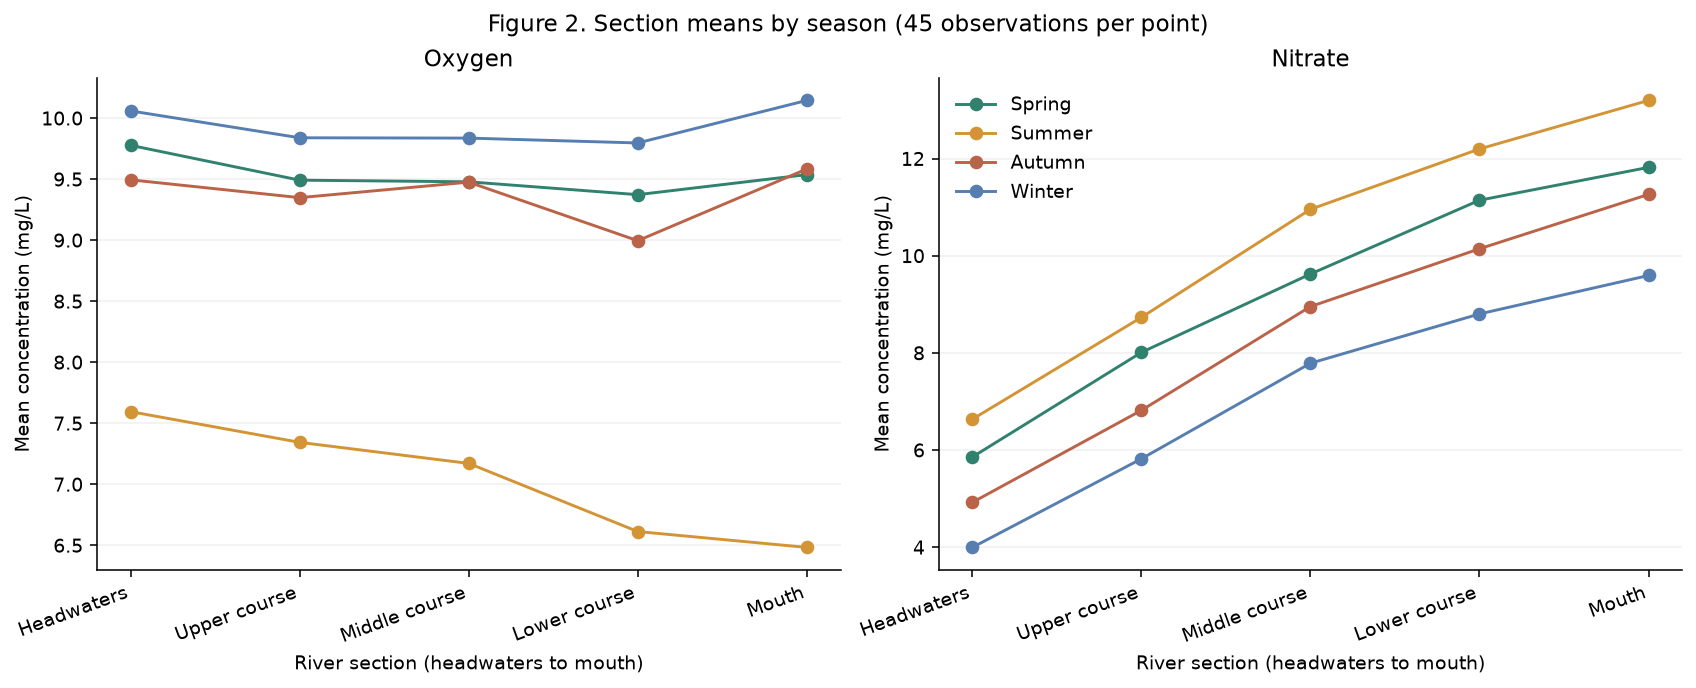
\includegraphics[width=\linewidth]{figures/section_season_means.png}
\caption{Section means by season; each point represents 45 observations. Connecting lines link ordered categories and do not fit a continuous spatial model.}\label{fig:spatial}
\end{figure}

Pooled section SDs include both seasonal variation and within-season variability. For this reason, they are not substituted for within-cell variances in the factorial contrasts. The inferential model estimates the 20 cell means and uses their residual variability. This preserves the observed balance while retaining different spatial patterns in different seasons.
